\chapter{Integer Values}


\textsc{Objectives}
\begin{tightlist}
\li Use integer literals
\li Use integer operators
\li Use associative and precedence rules to evaluate an integer
expression correctly
\li Use operators for integer values according to associative and
precedence rules
\li Write arithmetic expressions according to standard C++
practices
\end{tightlist}

In this set of notes, we will learn to print integer values and work with
some integer operators.

\newpage\section{Beyond hello world}

So far we have been printing textual data (i.e. C-strings) onto the console
window. It's time to do some math. We'll start off with whole numbers.


For this set of notes, instead of writing

\begin{console}
#include <iostream>
int main()
{
    std::cout << "Hello, world!" << std::endl;
    return 0;
}
\end{console}

I will write
\begin{console}
std::cout << "Hello, world!" << std::endl;
\end{console}

You should be smart enough to fill in the “surrounding” code:
\begin{console}
#include <iostream>
int main()
{
    std::cout << "Hello, world!" << std::endl;
    return 0;
}
\end{console}

By the way, it's a good practice to end your program output with a
newline.

\newpage\section{Printing integers}

An \EMPHASIZE{integer} is just whole number.

Try this:
\begin{console}
#include <iostream>
  
int main()
{
    std::cout << 42 << std::endl;
    std::cout << -5000 << std::endl;
    
    return 0;
}
\end{console}

Now this:
\begin{console}
#include <iostream>
  
int main()
{
    std::cout << 42 << -5000 << std::endl;
    
    return 0;
}
\end{console}

and then this:
\begin{console}
#include <iostream>
  
int main()
{
    std::cout << 42 << ", " << -5000 << std::endl;
    
    return 0;
}
\end{console}

AHA! So you can print integers and strings in the same print statement.

%
\begin{ex} 
  \label{ex:some-decision1}
  \tinysidebar{\debug{exercises/{empty0/question.tex}}}
  \solutionlink{sol:some-decision1}
  \qed
\end{ex} 
\begin{python0}
from solutions import *
add(label="ex:some-decision1",
    srcfilename='exercises/some-decision1/answer.tex') 
\end{python0}


%
\begin{ex} 
  \label{ex:some-decision1}
  \tinysidebar{\debug{exercises/{empty0/question.tex}}}
  \solutionlink{sol:some-decision1}
  \qed
\end{ex} 
\begin{python0}
from solutions import *
add(label="ex:some-decision1",
    srcfilename='exercises/some-decision1/answer.tex') 
\end{python0}


Here's an important jargon. Look at our program again:

\begin{console}
#include <iostream>
  
int main()
{
    std::cout << 42 << ", " << -5000 << std::endl;
    
    return 0;
}
\end{console}

The integer value 42 in the program is called an \EMPHASIZE{integer literal.}


Sometimes we also call this an \EMPHASIZE{integer constant.} The phrase
“in the program” is important. So if you're in your math classes, and you
write 42 in your assignment, you don't call that an integer literal!!!

\newpage\section{Integer operators: +, -, and *}

Now you might say, "Isn't this ..."
\begin{console}
std::cout << 42;
\end{console}
Now you might say, "Isn't this ..."
\begin{console}
std::cout << "42";
\end{console}

Yes. The \underline{output} is the same. But of course the \EMPHASIZE{value}
printed out in
the first program is an integer while the second is a string.

This will REALLY show you the difference. Try this:
\begin{console}
std::cout << 42 + 1 << std::endl;
std::cout << "42 + 1" << std::endl;
\end{console}

Get it?

Soooo ... C++ can do math!!!

Try this:
\begin{console}
std::cout << "42 + 1" << 42 + 1 << std::endl;
std::cout << "42 - 1" << 42 - 1 << std::endl;
std::cout << "2 * 3 = " << 2 * 3 << std::endl;
\end{console}

So far we see that C++ understands three \EMPHASIZE{operators}: +, –, and *.

No surprises there ... I hope!!!

You can (and should) think of the integer operator + as some kind of
machine that accepts two integer inputs and returns to you an integer
value:

\begin{center}
\begin{tikzpicture}
\node[draw,shape=rectangle,minimum size=2cm, inner sep=0](A) at (0, 0){+};
\node[draw=none,shape=rectangle,minimum size=2cm, inner sep=0](A1) at (0, 0.5){};
\node[draw=none,shape=rectangle,minimum size=2cm, inner sep=0](A2) at (0, -0.5){};
\node[draw=none,shape=circle,minimum size=1cm,inner sep=0](B) at (-3,0.5){};
\node[draw=none,shape=circle,minimum size=1cm,inner sep=0](C) at (-3, -0.5){};
\node[draw=none,shape=circle,minimum size=1cm,inner sep=0](D) at (3, 0){};

\draw[line width=0.04cm,black,->] (B) to  (A1);
\draw[line width=0.04cm,black,->] (C) to  (A2);
\draw[line width=0.04cm,black,->] (A) to  (D);


\end{tikzpicture}

\end{center}

And here's what happens when you put 42 and 1 into this machine:
\begin{center}
\begin{tikzpicture}
\node[draw,shape=rectangle,minimum size=2cm, inner sep=0](A) at (0, 0){+};
\node[draw=none,shape=rectangle,minimum size=2cm, inner sep=0](A1) at (0, 0.5){};
\node[draw=none,shape=rectangle,minimum size=2cm, inner sep=0](A2) at (0, -0.5){};
\node[draw=none,shape=circle,minimum size=1cm,inner sep=0](B) at (-3,0.5){};
\node[draw=none,shape=circle,minimum size=1cm,inner sep=0](C) at (-3, -0.5){};
\node[draw=none,shape=circle,minimum size=1cm,inner sep=0](D) at (3, 0){};

\node[anchor=east] at (1.7,0.5)   {43};

\node[anchor=east] at (-1.5,1)   {42};

\node[anchor=east] at (-1.5,-1)   {1};


\draw[line width=0.04cm,black,->] (B) to  (A1);
\draw[line width=0.04cm,black,->] (C) to  (A2);
\draw[line width=0.04cm,black,->] (A) to  (D);


\end{tikzpicture}

\end{center}

n C++, this operator + machine accepts integer inputs. There's another
operator + machine that accepts for instance numbers with decimal
places. The two are totally different machines. This is extremely
important. (I'll talk about numbers with decimal places in another set of
notes. These are called floating point numbers.) If I want to emphasize, I
will call the + in this set of notes, I will call it the
5 of 34 \EMPHASIZE{integer + operator}.

The story is very similar for operator - and *

%
\begin{ex} 
  \label{ex:some-decision1}
  \tinysidebar{\debug{exercises/{empty0/question.tex}}}
  \solutionlink{sol:some-decision1}
  \qed
\end{ex} 
\begin{python0}
from solutions import *
add(label="ex:some-decision1",
    srcfilename='exercises/some-decision1/answer.tex') 
\end{python0}


%
\begin{ex} 
  \label{ex:some-decision1}
  \tinysidebar{\debug{exercises/{empty0/question.tex}}}
  \solutionlink{sol:some-decision1}
  \qed
\end{ex} 
\begin{python0}
from solutions import *
add(label="ex:some-decision1",
    srcfilename='exercises/some-decision1/answer.tex') 
\end{python0}


\newpage\section{Integer operators: / and \%}

Division is ... well try this
\begin{console}
std::cout << "4 / 2 = " << 4 / 2 << std::endl;
\end{console}

And then this:
\begin{console}
std::cout << "100 / 20 = " << 100 / 20 << std::endl;
\end{console}

So far so good. No surprises.

BUT ... what about this program:
\begin{console}
std::cout << "9 / 3 = " << 9 / 3 << '\n'
          << "8 / 3 = " << 8 / 3 << '\n'
          << "7 / 3 = " << 7 / 3 << std::endl;
\end{console}
So you see what's happening?

If a and b are integer, then a / b gives the \EMPHASIZE{quotient} of a and b. This
is also called the \EMPHASIZE{integer division} of a by b. This is the same
as losing the fractional part of the usual mathematical division.

Let me repeat that again ...

In C++, 13 / 3 gives the \EMPHASIZE{integer part} of 13 divided by 3. In math, 13 divided by 3 is 4.333333... In C++, when / is used as an
operator for two \EMPHASIZE{integer} values in a C++ program, the result is an
\EMPHASIZE{integer}. So you lose the fractional part of the result from
mathematical division.

%
\begin{ex} 
  \label{ex:some-decision1}
  \tinysidebar{\debug{exercises/{empty0/question.tex}}}
  \solutionlink{sol:some-decision1}
  \qed
\end{ex} 
\begin{python0}
from solutions import *
add(label="ex:some-decision1",
    srcfilename='exercises/some-decision1/answer.tex') 
\end{python0}


\EMPHASIZE{REMEMBER THAT!}

When / is applied to two integers, we say that this division is an
\EMPHASIZE{integer division}. (Of course since we call this an integer
division operator you would expect the division operator in 1.123 / 3.2343
to be something totally different. We'll talk about this later.)
An integer division will produce an integer except for this case:

\begin{console}
std::cout << 1 / 0 << std::endl;
\end{console}

Run it. You will get an error. I hope that's not surprising! Division by zero
will cause an error. You already know that from your math classes: you
cannot divide by zero.

%
\begin{ex} 
  \label{ex:some-decision1}
  \tinysidebar{\debug{exercises/{empty0/question.tex}}}
  \solutionlink{sol:some-decision1}
  \qed
\end{ex} 
\begin{python0}
from solutions import *
add(label="ex:some-decision1",
    srcfilename='exercises/some-decision1/answer.tex') 
\end{python0}


Something like 10 + 55 is called an \EMPHASIZE{expression} (or integer
expression since it contains only integers). Here's another integer
expression:
\[ 10 + 55 + 412 – 12 * 43 – 67\]

Computing the resulting value of the expression is called
\EMPHASIZE{evaluating} the expression.

But what about the fractional part that's lost when doing an integer
division? What if you really wanted it?

Consider 13 / 3. C++ will give you 4. You're losing one-third. (Right?) In
math, the correct answer is 4 and one-third:

\[\frac{13}{3} = 4\frac{1}{3}\]

The 1 above is called the \EMPHASIZE{remainder}. Here's another example:

\[\frac{43}{8} = 5\frac{3}{8}\]

i.e., when 43 is divided by 8, you get 5 with a remainder of 3. What this
means is very simple. If you have 43 dollar bills and you want to give
them equally to your 8 good friends, then each will get 5 dollars and
you're left with 3 dollars. Let me repeat that – when you're given

\[\frac{43}{8}\]

then in order to write

\[\frac{43}{8} = 5\frac{3}{8}\]

the 5 is the integer division of 43 by 8 and the 3 is the remainder when
43 is divided by 8.

%
\begin{ex} 
  \label{ex:some-decision1}
  \tinysidebar{\debug{exercises/{empty0/question.tex}}}
  \solutionlink{sol:some-decision1}
  \qed
\end{ex} 
\begin{python0}
from solutions import *
add(label="ex:some-decision1",
    srcfilename='exercises/some-decision1/answer.tex') 
\end{python0}


irst of all you see that \% is an operator. What does the operator \% do?
Answer: 
\% is called the \EMPHASIZE{mod} operator.

%
\begin{ex} 
  \label{ex:some-decision1}
  \tinysidebar{\debug{exercises/{empty0/question.tex}}}
  \solutionlink{sol:some-decision1}
  \qed
\end{ex} 
\begin{python0}
from solutions import *
add(label="ex:some-decision1",
    srcfilename='exercises/some-decision1/answer.tex') 
\end{python0}


The integer quotient and remainder operators occur frequently in real life.
They are not just some fancy academic fluff. For instance suppose you
are told: “It took John 135 minutes to paint this wall,” but you prefer to
think in terms of hours and minutes. What would you do? You would do
this (mathematically):

\[\frac{135}{60} = 2\frac{15}{60}\]

i.e:

\begin{center}
  134 minutes = 2 hours and 15 minutes
\end{center}

To \underline{check} that this is correct:
\begin{center}
2 hours + 15 minutes\\
= 2 x 60 minutes + 15 minutes\\
= 120 minutes + 15 minutes\\
= 135 minutes
\end{center}

Correct? Of course the 2 is the integer quotient 135 / 60 (in C++) and the
15 is integer mod 135 \% 60 (in C++). And why do we quotient and mod
\underline{by 60}? Because 1 hour equals 60 minutes. Correct?

%
\begin{ex} 
  \label{ex:some-decision1}
  \tinysidebar{\debug{exercises/{empty0/question.tex}}}
  \solutionlink{sol:some-decision1}
  \qed
\end{ex} 
\begin{python0}
from solutions import *
add(label="ex:some-decision1",
    srcfilename='exercises/some-decision1/answer.tex') 
\end{python0}


if

\[\frac{192}{60} = 3\frac{12}{60}\]

But that's not the whole story. The remainder operator (i.e., the mod or
the \% operator) is in fact crucial to cryptography. Without it, e-commerce
would have been impossible. That's how important it really is. I bet your
high school teacher didn't tell you that.

%
\begin{ex} 
  \label{ex:some-decision1}
  \tinysidebar{\debug{exercises/{empty0/question.tex}}}
  \solutionlink{sol:some-decision1}
  \qed
\end{ex} 
\begin{python0}
from solutions import *
add(label="ex:some-decision1",
    srcfilename='exercises/some-decision1/answer.tex') 
\end{python0}

%
\begin{ex} 
  \label{ex:some-decision1}
  \tinysidebar{\debug{exercises/{empty0/question.tex}}}
  \solutionlink{sol:some-decision1}
  \qed
\end{ex} 
\begin{python0}
from solutions import *
add(label="ex:some-decision1",
    srcfilename='exercises/some-decision1/answer.tex') 
\end{python0}

%
\begin{ex} 
  \label{ex:some-decision1}
  \tinysidebar{\debug{exercises/{empty0/question.tex}}}
  \solutionlink{sol:some-decision1}
  \qed
\end{ex} 
\begin{python0}
from solutions import *
add(label="ex:some-decision1",
    srcfilename='exercises/some-decision1/answer.tex') 
\end{python0}

%
\begin{ex} 
  \label{ex:some-decision1}
  \tinysidebar{\debug{exercises/{empty0/question.tex}}}
  \solutionlink{sol:some-decision1}
  \qed
\end{ex} 
\begin{python0}
from solutions import *
add(label="ex:some-decision1",
    srcfilename='exercises/some-decision1/answer.tex') 
\end{python0}

%
\begin{ex} 
  \label{ex:some-decision1}
  \tinysidebar{\debug{exercises/{empty0/question.tex}}}
  \solutionlink{sol:some-decision1}
  \qed
\end{ex} 
\begin{python0}
from solutions import *
add(label="ex:some-decision1",
    srcfilename='exercises/some-decision1/answer.tex') 
\end{python0}

%
\begin{ex} 
  \label{ex:some-decision1}
  \tinysidebar{\debug{exercises/{empty0/question.tex}}}
  \solutionlink{sol:some-decision1}
  \qed
\end{ex} 
\begin{python0}
from solutions import *
add(label="ex:some-decision1",
    srcfilename='exercises/some-decision1/answer.tex') 
\end{python0}

%
\begin{ex} 
  \label{ex:some-decision1}
  \tinysidebar{\debug{exercises/{empty0/question.tex}}}
  \solutionlink{sol:some-decision1}
  \qed
\end{ex} 
\begin{python0}
from solutions import *
add(label="ex:some-decision1",
    srcfilename='exercises/some-decision1/answer.tex') 
\end{python0}


Remember this:
\begin{console}
std::cout << 5 \% 0 << std::endl;
\end{console}
Question: What are you to remember? And this too:
\begin{console}
std::cout << 5 / 0 << std::endl;
\end{console}

Using integer mod \% (and the integer quotient above) to convert from
minutes to hours and minutes might give you the impression that they
are use only for very trivial things. WRONG!!! Without the concept of
integer mod operator, we would not have the explosion of internet e-
commerce. Modern encryption (and many other things!!!) depends on the
concept of the integer mod operation.
Altogether we see that C++ understands five integer operators:
\begin{center}
  +     addition
  –     subtraction
  *     multiplication
  /     division (or quotient)
  \%     remainder
\end{center}
These operators are \EMPHASIZE{binary}
in the sense that you need to feed two
integers to the operator in order to get a result.

FOCUS! Read the above paragraphs again.

%
\begin{ex} 
  \label{ex:some-decision1}
  \tinysidebar{\debug{exercises/{empty0/question.tex}}}
  \solutionlink{sol:some-decision1}
  \qed
\end{ex} 
\begin{python0}
from solutions import *
add(label="ex:some-decision1",
    srcfilename='exercises/some-decision1/answer.tex') 
\end{python0}


You should thank the designers of C++ that they use the operator signs
+, – , *, / which you are used to, except for a slight change in meaning
to /. Whenever possible, programming language designers try to make
programming easier by using common mathematical notation and
convention.

\newpage\section{The dangerous $\land$ operator}

I want to give you \EMPHASIZE{a very important warning}.
You know from using your TI graphing calculator that $\land$ is used for
exponentiation. For instance if you want two-to-the-power-of-four, 2 4,
mathematically this is 2x2x2x2, you enter

\[
\texttt{2 $\land$ 4}
\]

into your calculator and it will spit out 16 for you. (Right?) Now run this
program:

\begin{console}
std::cout << (2 ^ 4) << std::endl;
\end{console}

When you run it ... it gives ... drumroll ...

\[6\]

and not 16!!! Whoa!!! Wassup???

The reason is not that C++ can't do exponentiation. In C++ the $\land$ has a
different meaning. We will talk about that much later. The important thing
to remember right now is that
\EMPHASIZE{$\land$ is not exponentiation in C++.}


%
\begin{ex} 
  \label{ex:some-decision1}
  \tinysidebar{\debug{exercises/{empty0/question.tex}}}
  \solutionlink{sol:some-decision1}
  \qed
\end{ex} 
\begin{python0}
from solutions import *
add(label="ex:some-decision1",
    srcfilename='exercises/some-decision1/answer.tex') 
\end{python0}

%
\begin{ex} 
  \label{ex:some-decision1}
  \tinysidebar{\debug{exercises/{empty0/question.tex}}}
  \solutionlink{sol:some-decision1}
  \qed
\end{ex} 
\begin{python0}
from solutions import *
add(label="ex:some-decision1",
    srcfilename='exercises/some-decision1/answer.tex') 
\end{python0}

%
\begin{ex} 
  \label{ex:some-decision1}
  \tinysidebar{\debug{exercises/{empty0/question.tex}}}
  \solutionlink{sol:some-decision1}
  \qed
\end{ex} 
\begin{python0}
from solutions import *
add(label="ex:some-decision1",
    srcfilename='exercises/some-decision1/answer.tex') 
\end{python0}


\newpage\section{Variables: input and output}

Try this:
\begin{console}
int x;
std::cin >> x;
std::cout << "x: " << x << '\n';
x = 42;
std::cout << "x: " << x << '\n';
\end{console}

When you run the program, enter an integer value on your keyboard and
press the Enter key.

variable – it holds a value and the value can vary. x is an integer
x is an \EMPHASIZE{integer variable}. x is a \EMPHASIZE{variable} because ... it's a
variable – it holds a value and the value can vary. x is an \EMPHASIZE{integer} because it can only hold an integer value. You have to create an
integer variable before you use it.

\sidenote{
  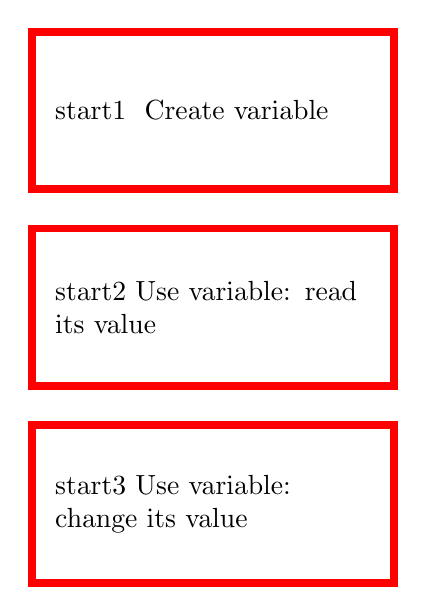
\begin{tikzpicture}
  \node[draw=red,text width=4cm,minimum height=2cm,minimum width=2cm, line width=0.1cm, inner sep=0.3cm] (a) at (2, 0) 
       {\tikzmark{start1} \normalsize{ Create variable}};
  \node[draw=red,text width=4cm,minimum height=2cm,minimum width=2cm, line width=0.1cm, inner sep=0.3cm] (a) at (2,-2.5) 
       {\tikzmark{start2} \normalsize{Use variable: read its value}};
  \node[draw=red,text width=4cm,minimum height=2cm,minimum width=2cm, line width=0.1cm, inner sep=0.3cm] (a) at (2,-5) 
       {\tikzmark{start3} \normalsize{Use variable: change its value}};
\end{tikzpicture}
}

\begin{console}[commandchars=\~\!\@]
int x; ~tikzmark!end1@
std::cin >> x;
std::cout << "x: " << x << '\n'; ~tikzmark!end2@
x = 42; ~tikzmark!end3@
std::cout << "x: " << x << '\n';
\end{console}
\DrawArrow[red, thick]{start1}{end1}
\DrawArrow[red, thick]{start2}{end2}
\DrawArrow[red, thick]{start3}{end3}

%
\begin{ex} 
  \label{ex:some-decision1}
  \tinysidebar{\debug{exercises/{empty0/question.tex}}}
  \solutionlink{sol:some-decision1}
  \qed
\end{ex} 
\begin{python0}
from solutions import *
add(label="ex:some-decision1",
    srcfilename='exercises/some-decision1/answer.tex') 
\end{python0}


It's not too surprising that you can do this:
\begin{console}
int x;
std::cin >> x;
std::cout << "x: " << x << '\n';
std::cout << "x + 1: " << x + 1 << '\n';
\end{console}

You can create more than one variable. Try this one:
\begin{console}
int x, y;
std::cin >> x;
std::cout << "x: " << x << '\n';
std::cout << "x + 1: " << x + 1 << '\n';
int z;
std::cin >> y >> z;
std::cout << "y + z: " << y + z << '\n';
\end{console}

I'll come back to variables again in more details ... there's a whole set of
notes on variables.

%
\begin{ex} 
  \label{ex:some-decision1}
  \tinysidebar{\debug{exercises/{empty0/question.tex}}}
  \solutionlink{sol:some-decision1}
  \qed
\end{ex} 
\begin{python0}
from solutions import *
add(label="ex:some-decision1",
    srcfilename='exercises/some-decision1/answer.tex') 
\end{python0}

%
\begin{ex} 
  \label{ex:some-decision1}
  \tinysidebar{\debug{exercises/{empty0/question.tex}}}
  \solutionlink{sol:some-decision1}
  \qed
\end{ex} 
\begin{python0}
from solutions import *
add(label="ex:some-decision1",
    srcfilename='exercises/some-decision1/answer.tex') 
\end{python0}


\newpage\section{A few simple facts: divisors and primes}

\textbf{{Divisors and Remainders}}

Divisors and primes and prime factorizations are already covered in
elementary algebra. Here's a quick review of some facts on divisors tied
in to C++.

An integer d is a \EMPHASIZE{divisor} of another n if d divides n. In other words an integer d is a divisor of n if you can find an integer x such that mathematically:
\[dx = n\]
For instance 3 is a divisor of 60 since mathematically
\[3x = 60\]
for x = 20. On the other hand 3 is not a divisor of 61 since you cannot find an \underline{integer} x satisfying
\[3x = 61\]
Another way to think of it is that

\EMPHASIZE{d is a divisor of n if the quotient of n
by d gives a 0 remainder}

i.e.,

\EMPHASIZE{d is a divisor of n if n \% d is 0}

For the case of 61, when you divide 61 by 3 you get
\[\frac{61}{3} = 20\frac{1}{3}\]
i.e, the remainder is 1 i.e.,
\[61 \% 3 is 1 which is not 0\]
So 3 is not a divisor of 61, or 61 is not divisible by 3.

%
\begin{ex} 
  \label{ex:some-decision1}
  \tinysidebar{\debug{exercises/{empty0/question.tex}}}
  \solutionlink{sol:some-decision1}
  \qed
\end{ex} 
\begin{python0}
from solutions import *
add(label="ex:some-decision1",
    srcfilename='exercises/some-decision1/answer.tex') 
\end{python0}

%
\begin{ex} 
  \label{ex:some-decision1}
  \tinysidebar{\debug{exercises/{empty0/question.tex}}}
  \solutionlink{sol:some-decision1}
  \qed
\end{ex} 
\begin{python0}
from solutions import *
add(label="ex:some-decision1",
    srcfilename='exercises/some-decision1/answer.tex') 
\end{python0}

%
\begin{ex} 
  \label{ex:some-decision1}
  \tinysidebar{\debug{exercises/{empty0/question.tex}}}
  \solutionlink{sol:some-decision1}
  \qed
\end{ex} 
\begin{python0}
from solutions import *
add(label="ex:some-decision1",
    srcfilename='exercises/some-decision1/answer.tex') 
\end{python0}


Of course you know that if you have something like this for positive
integer n:
\[n = dx\]
where d and x are positive integers greater than 1, you can think of that
as breaking up n into two pieces (or factors) d and x. You can continue to
do that for both d and x until you get the prime factorization of n. For
instance for n = 100,
\[100 = 4 x 25\]
This breaks up 100 into two factors 4 and 25. We now factorize 4 as
\[4 = 2x2\]
and so
\[100 = (2x2)x25\]
We are not done since we can factorize 25 as
\[25 = 5x5\]
This gives us the following factorization of 100:
\[100 = (2x2)x(5x5)\]
Since 2 and 5 are primes you can factorize them into smaller positive
integers greater than 1. So we get the prime factorization of 100:
\[100 = 2x2x5x5.\]
And you should know that the prime factorization of any positive integer
greater than 1 into primes is unique. For instance in the above example
we started with 100 and factorize 100 into 4x25. We then factorize 4 and
25 separately until we get
\[100 = 2x2x5x5.\]
If we started the factorization with 50x2 and then factorize 50 and 2
separately we will still arrive
\[50 = 2x5x5\]
and therefore
\[100 = 50x2 = (2x5x5)x2 = 2x5x5x2.\]
After you've organized the above prime factorizations in so that the terms
are ascending order we get
\[100 = 2x2x5x5\]
\[100 = 2x5x5x2 = 2x2x5x5\]
If I use exponentiation notation, I can write this:
\[100 = 2^2 x 5^2\]
Therefore no matter how you perform the prime factorization, after
rearranging the prime factors in ascending order, the prime factorization
is always the same. This fact is called the \EMPHASIZE{fundamental theorem of arithmetic} which states that ...

\EMPHASIZE{All positive integers can be expressed as a product of primes and, up to rearranging the primes, there is only one such prime factorization.}

%
\begin{ex} 
  \label{ex:some-decision1}
  \tinysidebar{\debug{exercises/{empty0/question.tex}}}
  \solutionlink{sol:some-decision1}
  \qed
\end{ex} 
\begin{python0}
from solutions import *
add(label="ex:some-decision1",
    srcfilename='exercises/some-decision1/answer.tex') 
\end{python0}

%
\begin{ex} 
  \label{ex:some-decision1}
  \tinysidebar{\debug{exercises/{empty0/question.tex}}}
  \solutionlink{sol:some-decision1}
  \qed
\end{ex} 
\begin{python0}
from solutions import *
add(label="ex:some-decision1",
    srcfilename='exercises/some-decision1/answer.tex') 
\end{python0}


Of course we just used the concept of primes. But what's a prime?

Here's a quick review. A \EMPHASIZE{prime} is a positive integer greater than 1 that is divisible only by 1 and itself. (Note that by definition 1 is not a prime.) For instance 13 is a prime. 42 on the other hand is not a prime since for instance 2 divides 42:
\[42 = 2 x 21\]

Of course 3 divides 42 as well since
\[42 = 3 x 14\]
But in order to say that 42 is not a prime, you only need to find one
positive divisor of 42 that is not 1 and not 42.

To check that 7 is a prime, you need to check
\begin{tightlist}
\li 2 is not a divisor of 7
\li is not a divisor of 7
\li is not a divisor of 7
\li is not a divisor of 7
\li is not a divisor of 7
\end{tightlist}
which is the same as checking:
\begin{tightlist}
\li The remainder when 7 divided by 2 is not 0
\li The remainder when 7 divided by 3 is not 0
\li The remainder when 7 divided by 4 is not 0
\li The remainder when 7 divided by 5 is not 0
\li The remainder when 7 divided by 6 is not 0
\end{tightlist}
which is the same as checking
\begin{tightlist}
\li 7 \% 2 is not 0
\li 7 \% 3 is not 0
\li 7 \% 4 is not 0
\li 7 \% 5 is not 0
\li 7 \% 6 is not 0
\end{tightlist}
Make sure you follow the above sequence of translations of prime
checking down to a sequence of % operator checks!!!

%
\begin{ex} 
  \label{ex:some-decision1}
  \tinysidebar{\debug{exercises/{empty0/question.tex}}}
  \solutionlink{sol:some-decision1}
  \qed
\end{ex} 
\begin{python0}
from solutions import *
add(label="ex:some-decision1",
    srcfilename='exercises/some-decision1/answer.tex') 
\end{python0}

To check if 11 is a prime, you will need to
\begin{tightlist}
\li 2 is not a divisor of 11
\li 3 is not a divisor of 11
\li 4 is not a divisor of 11
\li 5 is not a divisor of 11
\li 6 is not a divisor of 11
\li 7 is not a divisor of 11
\li 8 is not a divisor of 11
\li 9 is not a divisor of 11
\li 10 is not a divisor of 11
\end{tightlist}
Again, you're trying to hunt down a potential divisor of 11 between 2 and
10 (1 less than 11).

%
\begin{ex} 
  \label{ex:some-decision1}
  \tinysidebar{\debug{exercises/{empty0/question.tex}}}
  \solutionlink{sol:some-decision1}
  \qed
\end{ex} 
\begin{python0}
from solutions import *
add(label="ex:some-decision1",
    srcfilename='exercises/some-decision1/answer.tex') 
\end{python0}

%
\begin{ex} 
  \label{ex:some-decision1}
  \tinysidebar{\debug{exercises/{empty0/question.tex}}}
  \solutionlink{sol:some-decision1}
  \qed
\end{ex} 
\begin{python0}
from solutions import *
add(label="ex:some-decision1",
    srcfilename='exercises/some-decision1/answer.tex') 
\end{python0}


Now suppose we attempt to check if 35 is a prime, we would do the
same:
\begin{tightlist}
\li 35 \% 2 is $\textunderscore$ therefore 2 $\textunderscore$ (is or is not) a divisor of 35
\li 35 \% 3 is $\textunderscore$ therefore 3 $\textunderscore$ (is or is not) a divisor of 35
\li 35 \% 4 is $\textunderscore$ therefore 4 $\textunderscore$ (is or is not) a divisor of 35
\li 35 \% 5 is $\textunderscore$ therefore 5 $\textunderscore$ (is or is not) a divisor of 35
\li 35 \% 6 is $\textunderscore$ therefore 6 $\textunderscore$ (is or is not) a divisor of 35
\li 35 \% 7 is $\textunderscore$ therefore 7 $\textunderscore$ (is or is not) a divisor of 35
\li etc.
\end{tightlist}
WAIT!!!! HOLD YOUR HORSES!!!

When we were testing integer division by 5, you see that 35 % 5 is 0.
This means that 5 is a divisor of 35. That means that 35 is (already) not
a prime. There's no point in continuing the checks!!! I should have
stopped then!!! Why waste time?!?


%
\begin{ex} 
  \label{ex:some-decision1}
  \tinysidebar{\debug{exercises/{empty0/question.tex}}}
  \solutionlink{sol:some-decision1}
  \qed
\end{ex} 
\begin{python0}
from solutions import *
add(label="ex:some-decision1",
    srcfilename='exercises/some-decision1/answer.tex') 
\end{python0}

%
\begin{ex} 
  \label{ex:some-decision1}
  \tinysidebar{\debug{exercises/{empty0/question.tex}}}
  \solutionlink{sol:some-decision1}
  \qed
\end{ex} 
\begin{python0}
from solutions import *
add(label="ex:some-decision1",
    srcfilename='exercises/some-decision1/answer.tex') 
\end{python0}


\newpage\section{Coding style for expressions}

For binary operators:
BAD:
\begin{console}
123+13-32*234/23\%228
\end{console}
BAD:
\begin{console}
123+ 13 -32*    234/    23    \%228
\end{console}
GOOD
\begin{console}
123 + 13 – 32 * 234 / 23 \% 228
\end{console}
Enough said.


For unary operators:

BAD
\begin{console}
+ 123 + + 13 - – 32 * 234
\end{console}
GOOD
\begin{console}
+123 + +13 - -32 * 234
\end{console}
Enough said.


Incidentally, you cannot write this:
\begin{console}
+123 ++ 13 -- 32 * 234
\end{console}

Because ++ and -- have special meanings in C++. We'll talk about that
later.

\newpage\section{A few simple facts: 10}

There's something special about integer division by 10 and mod 10.


Try this:
\begin{console}
std::cout << "1358 / 10 = " << 1358 / 10 <<std::endl;
\end{console}


You notice that 1358 / 10 is just 1358 with its rightmost digit chopped off,
i.e., it's 135.


That makes sense right? Mathematically 1358 divided by 10 gives 135.8.
So in C++, since you only get the integer part of the division, the integer
division 1358 / 10 is 135.


%
\begin{ex} 
  \label{ex:some-decision1}
  \tinysidebar{\debug{exercises/{empty0/question.tex}}}
  \solutionlink{sol:some-decision1}
  \qed
\end{ex} 
\begin{python0}
from solutions import *
add(label="ex:some-decision1",
    srcfilename='exercises/some-decision1/answer.tex') 
\end{python0}


%
\begin{ex} 
  \label{ex:some-decision1}
  \tinysidebar{\debug{exercises/{empty0/question.tex}}}
  \solutionlink{sol:some-decision1}
  \qed
\end{ex} 
\begin{python0}
from solutions import *
add(label="ex:some-decision1",
    srcfilename='exercises/some-decision1/answer.tex') 
\end{python0}


%
\begin{ex} 
  \label{ex:some-decision1}
  \tinysidebar{\debug{exercises/{empty0/question.tex}}}
  \solutionlink{sol:some-decision1}
  \qed
\end{ex} 
\begin{python0}
from solutions import *
add(label="ex:some-decision1",
    srcfilename='exercises/some-decision1/answer.tex') 
\end{python0}


%
\begin{ex} 
  \label{ex:some-decision1}
  \tinysidebar{\debug{exercises/{empty0/question.tex}}}
  \solutionlink{sol:some-decision1}
  \qed
\end{ex} 
\begin{python0}
from solutions import *
add(label="ex:some-decision1",
    srcfilename='exercises/some-decision1/answer.tex') 
\end{python0}


%
\begin{ex} 
  \label{ex:some-decision1}
  \tinysidebar{\debug{exercises/{empty0/question.tex}}}
  \solutionlink{sol:some-decision1}
  \qed
\end{ex} 
\begin{python0}
from solutions import *
add(label="ex:some-decision1",
    srcfilename='exercises/some-decision1/answer.tex') 
\end{python0}


%
\begin{ex} 
  \label{ex:some-decision1}
  \tinysidebar{\debug{exercises/{empty0/question.tex}}}
  \solutionlink{sol:some-decision1}
  \qed
\end{ex} 
\begin{python0}
from solutions import *
add(label="ex:some-decision1",
    srcfilename='exercises/some-decision1/answer.tex') 
\end{python0}


%
\begin{ex} 
  \label{ex:some-decision1}
  \tinysidebar{\debug{exercises/{empty0/question.tex}}}
  \solutionlink{sol:some-decision1}
  \qed
\end{ex} 
\begin{python0}
from solutions import *
add(label="ex:some-decision1",
    srcfilename='exercises/some-decision1/answer.tex') 
\end{python0}


%
\begin{ex} 
  \label{ex:some-decision1}
  \tinysidebar{\debug{exercises/{empty0/question.tex}}}
  \solutionlink{sol:some-decision1}
  \qed
\end{ex} 
\begin{python0}
from solutions import *
add(label="ex:some-decision1",
    srcfilename='exercises/some-decision1/answer.tex') 
\end{python0}


The above exercises are important: Extracting data from data is very
common in Computer Science (well ... it's important in every area of
Science). For instance google extracts keywords from web pages for
indexing so that when someone does search for that word, google can
return the web page's URL quickly. But that's slightly different from our
case since google extracts data from strings and not integers.


The above involves \underline{cutting out} digits of chunks of digits from an integer
value. You can \underline{build} integer values using chunks of integers. For
instance you know from your math classes that
\[1358\]
is the same as (using mathematical notation):
\[1\times1000 + 3\times100 + 5\times10 + 8\times1\]
In this case, you are constructing 1358 using the digits 1, 3, 5 and 8
together with powers of 10. (Don't forget that 1 is a power of 10 too ...
10$^0$ = 1. Correct?)

%
\begin{ex} 
  \label{ex:some-decision1}
  \tinysidebar{\debug{exercises/{empty0/question.tex}}}
  \solutionlink{sol:some-decision1}
  \qed
\end{ex} 
\begin{python0}
from solutions import *
add(label="ex:some-decision1",
    srcfilename='exercises/some-decision1/answer.tex') 
\end{python0}


Note that multiplying a number with a power of 10 is the same as adding
a certain number of zeroes to the left of the given number. For instance
in the above,
\[3\times100 = 300\]
i.e., multiplication by 100 just adds 2 zeroes to the given number. Here's
another example:
\[8 \times 10000 = 80000\]
This works not just for digits (of course). For instance
\[867 \times 100000 = 86700000\]

%
\begin{ex} 
  \label{ex:some-decision1}
  \tinysidebar{\debug{exercises/{empty0/question.tex}}}
  \solutionlink{sol:some-decision1}
  \qed
\end{ex} 
\begin{python0}
from solutions import *
add(label="ex:some-decision1",
    srcfilename='exercises/some-decision1/answer.tex') 
\end{python0}


%
\begin{ex} 
  \label{ex:some-decision1}
  \tinysidebar{\debug{exercises/{empty0/question.tex}}}
  \solutionlink{sol:some-decision1}
  \qed
\end{ex} 
\begin{python0}
from solutions import *
add(label="ex:some-decision1",
    srcfilename='exercises/some-decision1/answer.tex') 
\end{python0}

%
\begin{ex} 
  \label{ex:some-decision1}
  \tinysidebar{\debug{exercises/{empty0/question.tex}}}
  \solutionlink{sol:some-decision1}
  \qed
\end{ex} 
\begin{python0}
from solutions import *
add(label="ex:some-decision1",
    srcfilename='exercises/some-decision1/answer.tex') 
\end{python0}


%
\begin{ex} 
  \label{ex:some-decision1}
  \tinysidebar{\debug{exercises/{empty0/question.tex}}}
  \solutionlink{sol:some-decision1}
  \qed
\end{ex} 
\begin{python0}
from solutions import *
add(label="ex:some-decision1",
    srcfilename='exercises/some-decision1/answer.tex') 
\end{python0}

%
\begin{ex} 
  \label{ex:some-decision1}
  \tinysidebar{\debug{exercises/{empty0/question.tex}}}
  \solutionlink{sol:some-decision1}
  \qed
\end{ex} 
\begin{python0}
from solutions import *
add(label="ex:some-decision1",
    srcfilename='exercises/some-decision1/answer.tex') 
\end{python0}


%
\begin{ex} 
  \label{ex:some-decision1}
  \tinysidebar{\debug{exercises/{empty0/question.tex}}}
  \solutionlink{sol:some-decision1}
  \qed
\end{ex} 
\begin{python0}
from solutions import *
add(label="ex:some-decision1",
    srcfilename='exercises/some-decision1/answer.tex') 
\end{python0}

%
\begin{ex} 
  \label{ex:some-decision1}
  \tinysidebar{\debug{exercises/{empty0/question.tex}}}
  \solutionlink{sol:some-decision1}
  \qed
\end{ex} 
\begin{python0}
from solutions import *
add(label="ex:some-decision1",
    srcfilename='exercises/some-decision1/answer.tex') 
\end{python0}


%
\begin{ex} 
  \label{ex:some-decision1}
  \tinysidebar{\debug{exercises/{empty0/question.tex}}}
  \solutionlink{sol:some-decision1}
  \qed
\end{ex} 
\begin{python0}
from solutions import *
add(label="ex:some-decision1",
    srcfilename='exercises/some-decision1/answer.tex') 
\end{python0}

%
\begin{ex} 
  \label{ex:some-decision1}
  \tinysidebar{\debug{exercises/{empty0/question.tex}}}
  \solutionlink{sol:some-decision1}
  \qed
\end{ex} 
\begin{python0}
from solutions import *
add(label="ex:some-decision1",
    srcfilename='exercises/some-decision1/answer.tex') 
\end{python0}


%
\begin{ex} 
  \label{ex:some-decision1}
  \tinysidebar{\debug{exercises/{empty0/question.tex}}}
  \solutionlink{sol:some-decision1}
  \qed
\end{ex} 
\begin{python0}
from solutions import *
add(label="ex:some-decision1",
    srcfilename='exercises/some-decision1/answer.tex') 
\end{python0}


\newpage\section{A few simple facts: evenness/oddness}

Another thing you should be aware of is the following:

First any integer \% 5 is either 0 or 1 or 2 or 3 or 4. Right?

In general, if n is a positive integer, then any integer \% n is either 0 or 1
or 2 or ... or n - 1.

In particular any integer \% 2 is either 0 or 1. Note that an integer is even
if its mod 2 is 0. Otherwise it's odd.

Try this:
\begin{console}
std::cout << 5 % 2 << std::endl;
std::cout << 6 % 2 << std::endl;
\end{console}

Get it?

\newpage\section{Associativity and precedence}



College Algebra is a prerequisite. So you know what I mean by
associativity and operator precedence right? Yes? No?


All the operators you saw (+, -, *, /, \%) are binary operators in the sense
that for instance + is applied to two values. For example we have 2 + 3.


\textbf{Associativity.}

Now think about this integer expression:
\[2+3+1\]
What we really mean is
\[(2 + 3) + 1\]
As you can see with the parentheses, each + is applied to two numbers.
\begin{console}
\li The left + is applied to 2 and 3.
\li The right + is applied to (2+3) and 1, i.e., 5 and 1.
\end{console}
Correct?


But wait. There's another way to do it:
\[2 + (3 + 1)\]

So is 2 + 3 + 1
\[(2 + 3) + 1 \text{     or     } 2 + (3 + 1)\text{    ???}\]
Of course it doesn't matter!!! Ultimately they both evaluate to the same value:

\begin{align*}
&(2 + 3) + 1 & & 2 + (3 + 1)\\
&=5+1 & & =2+4\\
&=6 & & =6
\end{align*}

But this is not the case for all operators. For instance, consider the minus
operator:
\begin{align*}
&(2 - 3) - 1 & & 2 - (3 - 1)\\
&=-1 - 1 & & =2-2\\
&=-2 & & =0
\end{align*}

Long time ago, mathematicians decided that they are too efficient to write
\[(2 + 3) + 1\]
So they got together and come to an agreement that if parentheses are
left out for a string of pluses, you always do the pluses from left to right.
We say that \textbf{{+ associates left-to-right or associates to the right.}} So
\[1+2+3+4\]
is really a shorthand for
\[((1 + 2) + 3) + 4\]
The important thing to remember is that whether + is left or right
associated is a matter of convention.

+, –, *, /, \% associates from left to right. So for instance if I write
\[3–4–5–2\]
I mean
\[((3 – 4) – 5) – 2\]
i.e. do the leftmost subtraction first.


\textbf{{Precedence Rules}}

What about the case where you have not just pluses? What about
something like
\[1+3–2*6/3*4+6\]
In C++, you determine which operator goes first using this table:

\noindent\fbox{\begin{minipage}{\textwidth}
    \begin{align*}
      &() & &\text{first priority}\\
      &*, /, \% & &\text{second priority}\\
      &+, - & &\text{third priority}
    \end{align*}
\end{minipage}}

Remember PEMDAS from your math classes? Note the difference is that
* and / are at the same level, and + and – are at the same level.

%
\begin{ex} 
  \label{ex:some-decision1}
  \tinysidebar{\debug{exercises/{empty0/question.tex}}}
  \solutionlink{sol:some-decision1}
  \qed
\end{ex} 
\begin{python0}
from solutions import *
add(label="ex:some-decision1",
    srcfilename='exercises/some-decision1/answer.tex') 
\end{python0}


It will be clearer when I do an example. So let's evaluate the above
expression:
\[1+3–2*6/3*4+6\]
When we check the priority table, we don't see parentheses, i.e., there's
nothing for the first priority. What about the second priority operators? I
do see * and /. So let's do them. Don't forget that these associate left-to-
right which is just a fancy way of saying “do the leftmost first and keep
moving right”. You see that for * and / (i.e., ignore + and – for now), the
first to occur is the * here:
\[1+3–\underline{2*6}/ 3*4+6\]
So let's do that:
\begin{align*}
  &1+3–\underline{2*6}/ 3*4+6\\
  &= 1 + 3 – 12 / 3 * 4 + 6 & &i.e., 2 * 6 = 12
\end{align*}
The next in the second priority operators is here:
\[1 + 3 – \underline{12 / 3} * 4 + 6\]
Let's do that:
\begin{align*}
  &1 + 3 – \underline{12 / 3} * 4 + 6\\
  &=1+3–4*4+6 & &i.e., 12 * 3 = 4
\end{align*}
Got it?

And the last evaluation for the second priority operators give us this:
\begin{align*}
&1+3–\underline{4*4}+6\\
&= 1 + 3 – 16 + 6 & &i.e., 4 * 4 = 16
  \end{align*}
    
There are now no more second priority operators. Let's move on to the
third priority operators, i.e., the + and the –. Here we go:
\begin{align*}
  &\underline{1 + 3} – 16 + 6 \\
  &= \underline{4 – 16} + 6 & &i.e., 1 + 3 = 4 \\
  &= \underline{–12 + 6} & &i.e., 4 – 16 = -12 \\
  &= –6 & &i.e., -12 + 6 = -12
\end{align*}
Don't forget that + and – associates left-to-right. So we have to always
pick + and – going left-to-right.

That's all there is to it. If I put all the computations together this is what I
get:
\begin{align*}
  &1+3–\underline{2*6}/ 3*4+6 \\
  &= 1 + 3 – \underline{12 / 3} * 4 + 6 & &i.e., 2 * 6 = 12\\
  &=1+3–\underline{4*4}+6 & &i.e., 12/ 3 = 4\\
  &= \underline{1 + 3} – 16 + 6 & &i.e., 4 * 4 = 16\\
  &= \underline{4 – 16} + 6 & &i.e., 1 + 3 = 4\\
  &= \underline{–12 + 6} & &i.e., 4 – 16 = -12\\
  &= –6 & &i.e., -12 + 6 = -12\\
\end{align*}

%
\begin{ex} 
  \label{ex:some-decision1}
  \tinysidebar{\debug{exercises/{empty0/question.tex}}}
  \solutionlink{sol:some-decision1}
  \qed
\end{ex} 
\begin{python0}
from solutions import *
add(label="ex:some-decision1",
    srcfilename='exercises/some-decision1/answer.tex') 
\end{python0}


Associative and precedence are extremely important because performing
computations in different orders can lead to different results. If you do it
in the wrong order, then ... that's BAD! Just imagine the collapse of
financial institutions or random explosions of missiles/shuttles because of
a misunderstanding of the way C++ computes value!!!


Fortunately C++ is designed so that computations done in the computer
follows the standard associative and precedence rules.

%
\begin{ex} 
  \label{ex:some-decision1}
  \tinysidebar{\debug{exercises/{empty0/question.tex}}}
  \solutionlink{sol:some-decision1}
  \qed
\end{ex} 
\begin{python0}
from solutions import *
add(label="ex:some-decision1",
    srcfilename='exercises/some-decision1/answer.tex') 
\end{python0}

%
\begin{ex} 
  \label{ex:some-decision1}
  \tinysidebar{\debug{exercises/{empty0/question.tex}}}
  \solutionlink{sol:some-decision1}
  \qed
\end{ex} 
\begin{python0}
from solutions import *
add(label="ex:some-decision1",
    srcfilename='exercises/some-decision1/answer.tex') 
\end{python0}

%
\begin{ex} 
  \label{ex:some-decision1}
  \tinysidebar{\debug{exercises/{empty0/question.tex}}}
  \solutionlink{sol:some-decision1}
  \qed
\end{ex} 
\begin{python0}
from solutions import *
add(label="ex:some-decision1",
    srcfilename='exercises/some-decision1/answer.tex') 
\end{python0}



Let's try another example, this time an expression with a pair of
parentheses:
\[3 + 1 * 4 – 4 * 3 * 2 / (2 + 6 * 2 – 1) + 6 * 7\]
In this case, there's one pair of parentheses. So we have to evaluate the
expression within the parentheses first. In the parentheses, there are no
parentheses, i.e., there are no priority one operators. So we look for
priority two operators: * and /. There is one. So we evaluate that
operator:
\begin{align*}
  &3 + 1 * 4 – 4 * 3 * 2 / (2 + \underline{6 * 2} – 1) + 6 * 7\\
  &= 3 + 1 * 4 – 4 * 3 * 2 / (2 + 12 – 1) + 6 * 7 & &i.e., 6 * 2 = 12
\end{align*}
To make it easier to follow, I've underlined the expression I'm evaluating.

There are no priority two operators. So we look for priority 3 operators,
i.e., + and –. There are two so we do this going left-to-right:
\begin{align*}
&3 + 1 * 4 – 4 * 3 * 2 / (\underline{2 + 12} – 1) + 6 * 7\\
&= 3 + 1 * 4 – 4 * 3 * 2 / (\underline{14 – 1}) + 6 * 7 & &i.e., 2 + 12 = 14\\
&= 3 + 1 * 4 – 4 * 3 * 2 / (13) + 6 * 7 & &i.e., 14 – 1 = 13\\
&= 3 + 1 * 4 – 4 * 3 * 2 / 13 + 6 * 7 & &i.e., (13) = 13
\end{align*}
(In the last step we just remove the useless parentheses.) Now there are
no parentheses (priority one). So look for priority two operators and
evaluate them left-to-right:
\begin{align*}
&3 + 1 * 4 – 4 * 3 * 2 / 13 + 6 * 7\\
&= 3 + 4 – 4 * 3 * 2 / 13 + 6 * 7 & &i.e., 1 * 4 = 4\\
&= 3 + 4 – 12 * 2 / 13 + 6 * 7 & &i.e., 4 * 3 = 12\\
&= 3 + 4 – 24 / 13 + 6 * 7 & &i.e., 12 * 2 = 24\\
&=3+4–1+6*7 & &i.e., 24 / 13 = 1\\
&= 3 + 4 – 1 + 42 & &i.e., 6 * 7 = 42
\end{align*}

Don't forget that in the fourth line, 24/13 = 1 because we're doing C++
integer quotient, not real number division in college algebra.
Now there are no more priority two operators. We evaluate the priority
three operators, i.e., the + and –.
\begin{align*}
&3 + 4 – 1 + 42\\
&= 7 – 1 + 42 & &i.e., 3 + 4 = 7\\
= 6 + 42 & &i.e., 7 – 1 = 6\\
= 48 & &i.e., 6 + 42 = 48
\end{align*}
and we're done.
Study every single step of the above computation.

%
\begin{ex} 
  \label{ex:some-decision1}
  \tinysidebar{\debug{exercises/{empty0/question.tex}}}
  \solutionlink{sol:some-decision1}
  \qed
\end{ex} 
\begin{python0}
from solutions import *
add(label="ex:some-decision1",
    srcfilename='exercises/some-decision1/answer.tex') 
\end{python0}

%
\begin{ex} 
  \label{ex:some-decision1}
  \tinysidebar{\debug{exercises/{empty0/question.tex}}}
  \solutionlink{sol:some-decision1}
  \qed
\end{ex} 
\begin{python0}
from solutions import *
add(label="ex:some-decision1",
    srcfilename='exercises/some-decision1/answer.tex') 
\end{python0}

%
\begin{ex} 
  \label{ex:some-decision1}
  \tinysidebar{\debug{exercises/{empty0/question.tex}}}
  \solutionlink{sol:some-decision1}
  \qed
\end{ex} 
\begin{python0}
from solutions import *
add(label="ex:some-decision1",
    srcfilename='exercises/some-decision1/answer.tex') 
\end{python0}

%
\begin{ex} 
  \label{ex:some-decision1}
  \tinysidebar{\debug{exercises/{empty0/question.tex}}}
  \solutionlink{sol:some-decision1}
  \qed
\end{ex} 
\begin{python0}
from solutions import *
add(label="ex:some-decision1",
    srcfilename='exercises/some-decision1/answer.tex') 
\end{python0}


f you have an expression with \underline{two} separate pairs of parentheses such
as:
\[2 * (3 + 5) – 3 * (5 + 3 * 2)\]
you should present your answer by evaluating left-to-right, i.e., evaluate
the leftmost parentheses first.
\begin{align*}
&2 * (3 + 5) – 3 * (5 + 3 * 2)
&= 2 * (8) – 3 * (5 + 3 * 2) & &i.e., 3 + 5 = 8\\
&= 2 * 8 – 3 * (5 + 3 * 2) & &i.e., (8) = 8\\
&= 2 * 8 – 3 * (5 + 6) & &i.e., 3 * 2 = 6\\
&= 2 * 8 – 3 * (11) & &i.e., 5 + 6 = 11 \\
&= 2 * 8 – 3 * 11 & &i.e., (11) = 11 \\
&= 16 – 3 * 11 & &i.e., 2 * 8 = 16\\
= 16 – 33 & &i.e., 3 * 11\\
= -17 & &i.e., 16 – 33 = -17
\end{align*}

%
\begin{ex} 
  \label{ex:some-decision1}
  \tinysidebar{\debug{exercises/{empty0/question.tex}}}
  \solutionlink{sol:some-decision1}
  \qed
\end{ex} 
\begin{python0}
from solutions import *
add(label="ex:some-decision1",
    srcfilename='exercises/some-decision1/answer.tex') 
\end{python0}

%
\begin{ex} 
  \label{ex:some-decision1}
  \tinysidebar{\debug{exercises/{empty0/question.tex}}}
  \solutionlink{sol:some-decision1}
  \qed
\end{ex} 
\begin{python0}
from solutions import *
add(label="ex:some-decision1",
    srcfilename='exercises/some-decision1/answer.tex') 
\end{python0}


You can also have situations when parentheses are nested like this:
\[1 + (\underline{2 * 1 + (3 + 4 * 5) / 2}) + 5\]
i.e., within a pair of parentheses, you see another pair. As you're
evaluating the first pair of parentheses, you have to apply the priority
rules, which means you have to evaluate the inner parentheses first.
That's all.
\begin{align*}
  &1 + (2 * 1 + (3 + \underline{4 * 5}) / 2) + 5\\
  &= 1 + (2 * 1 + (\underline{3 + 20}) / 2) + 5 & &i.e., 4 * 5 = 20\\
  &= 1 + (2 * 1 + \underline{(23)} / 2) + 5 & &i.e., 3 + 20 = 23\\
  &= 1 + (\underline{2 * 1} + 23 / 2) + 5 & &i.e., (23) = 23\\
  &= 1 + (2 + \underline{23 / 2}) + 5 & &i.e., 2 * 1 = 2\\
  &= 1 + (\underline{2 + 11}) + 5 & &i.e., 23/ 2 = 11\\
  &= 1 + \underline{(13)} + 5 & &i.e., 2 + 11 = 13\\
  &= \underline{1 + 13} + 5 & &i.e., (13) = 13\\
  &= \underline{14 + 5} & &i.e., 14 + 5 = 19\\
  &= 19
\end{align*}

%
\begin{ex} 
  \label{ex:some-decision1}
  \tinysidebar{\debug{exercises/{empty0/question.tex}}}
  \solutionlink{sol:some-decision1}
  \qed
\end{ex} 
\begin{python0}
from solutions import *
add(label="ex:some-decision1",
    srcfilename='exercises/some-decision1/answer.tex') 
\end{python0}

%
\begin{ex} 
  \label{ex:some-decision1}
  \tinysidebar{\debug{exercises/{empty0/question.tex}}}
  \solutionlink{sol:some-decision1}
  \qed
\end{ex} 
\begin{python0}
from solutions import *
add(label="ex:some-decision1",
    srcfilename='exercises/some-decision1/answer.tex') 
\end{python0}

%
\begin{ex} 
  \label{ex:some-decision1}
  \tinysidebar{\debug{exercises/{empty0/question.tex}}}
  \solutionlink{sol:some-decision1}
  \qed
\end{ex} 
\begin{python0}
from solutions import *
add(label="ex:some-decision1",
    srcfilename='exercises/some-decision1/answer.tex') 
\end{python0}

%
\begin{ex} 
  \label{ex:some-decision1}
  \tinysidebar{\debug{exercises/{empty0/question.tex}}}
  \solutionlink{sol:some-decision1}
  \qed
\end{ex} 
\begin{python0}
from solutions import *
add(label="ex:some-decision1",
    srcfilename='exercises/some-decision1/answer.tex') 
\end{python0}

%
\begin{ex} 
  \label{ex:some-decision1}
  \tinysidebar{\debug{exercises/{empty0/question.tex}}}
  \solutionlink{sol:some-decision1}
  \qed
\end{ex} 
\begin{python0}
from solutions import *
add(label="ex:some-decision1",
    srcfilename='exercises/some-decision1/answer.tex') 
\end{python0}

%
\begin{ex} 
  \label{ex:some-decision1}
  \tinysidebar{\debug{exercises/{empty0/question.tex}}}
  \solutionlink{sol:some-decision1}
  \qed
\end{ex} 
\begin{python0}
from solutions import *
add(label="ex:some-decision1",
    srcfilename='exercises/some-decision1/answer.tex') 
\end{python0}



\newpage\section{Unary and binary operators}
An operator is \EMPHASIZE{binary} if it is applied to two values. For instance the +
in the following expression:
\[2+3\]
is binary. You have already seen the binary +, –,*,/,\%. They all require
two values to make sense.

There are actually two operators that require only one value. These are \EMPHASIZE{unary} operators. The unary + operator (the “positive” operator)
appears in this expression:

\sidenote{
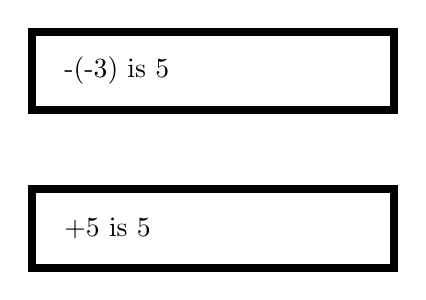
\begin{tikzpicture}
  \node[draw,text width=4cm,minimum height=1cm,minimum width=1cm, line width=0.1cm, inner sep=0.3cm] at (2,-2)
       {\normalsize{ +5 is 5}};
       
  \node[draw,text width=4cm,minimum height=1cm,minimum width=1cm, line width=0.1cm, inner sep=0.3cm] at (2,0)
       {\normalsize{ -(-3) is 5}};
\end{tikzpicture}
}


\[+2\]
and of course there's the unary – operator (the “negative” operator):
\[–2\]
So the symbol + and – have two different meanings.

Now we need to modify the chart of precedence rules:

  
\noindent\fbox{\begin{minipage}{\textwidth}
    \begin{align*}
      &() & &\text{first priority}\\
      &*, /, \% & &\text{second priority}\\
      &+, - & &\text{third priority}
    \end{align*}
\end{minipage}}

%
\begin{ex} 
  \label{ex:some-decision1}
  \tinysidebar{\debug{exercises/{empty0/question.tex}}}
  \solutionlink{sol:some-decision1}
  \qed
\end{ex} 
\begin{python0}
from solutions import *
add(label="ex:some-decision1",
    srcfilename='exercises/some-decision1/answer.tex') 
\end{python0}


Try this example involving three unary – operators (the “negative”
operator):
\begin{console}
std::cout << - - - 2;
\end{console}
You should get -2. Right? If you try to put parentheses in the expression,
of course the only reasonable way to do it would be like this:
-\[(-(-2))\]
I mean ... what else can it be??? You can't do this: (((-)-)2)!!! It has
no meaning at all!!!
In other words you apply the rightmost – first. The last – is the leftmost.
The unary – operator associates right to left. It's the same for the unary +
operator (“positive” operator).


\newpage\section{Summary}

You can think of an operator as something that will give you a value.
A binary operator is an operator that produces a value when you feed it
two values.
A unary operator is an operator that produces a value when you feed it
one value.
An operator is an integer operator if it produces an integer value.
C++ understands the following binary integer operator:
\begin{align*}
&+ & &addition\\
&– & &subtraction\\
&* & &multiplication\\
&/ & &division\\
&\% & &remainder
\end{align*}
and the following unary operators:

\begin{align*}
&+ & &positive\\
&– & &negative
\end{align*}

Here are the precedence rules for the operators:

\noindent\fbox{\begin{minipage}{\textwidth}
    \begin{align*}
      &() & &\text{first priority}\\
      &*, /, \% & &\text{second priority}\\
      &+, - & &\text{third priority}
    \end{align*}
\end{minipage}}
The binary integer operators associates left-to-right. The unary integer
operators associates right-to-left. So for example:
\begin{align*}
&1+2–3+4 &\text{is} & &((1 + 2) – 3) + 4\\
\text{and}\\
&-+-1 &\text{is} & &-(+(-1))
\end{align*}
You can print integer values in a print statement:
\[std::cout << 42 << std::endl;\]
You can mix the printing of integer, string values, and character values:
std::cout << 1 << ", " << 2 << "buckle my shoe"
<< '!' << std::endl;
When you print an expression, the evaluated expression is printed:
\[std::cout << 40 + 1 + 1 << std::endl;\]
